\section{Problema físico}\label{secao_desc_prob}
\subsection{Descrição}

O problema físico em regime permanente considerado neste trabalho é baseado no problema proposto por \cite{reciproc_3} e \cite{artigo_abreu_3},
e a geometria do arranjo físico correspondente está apresentada na figura \ref{fig2}. 
\begin{figure}[h!b]
\begin{center}
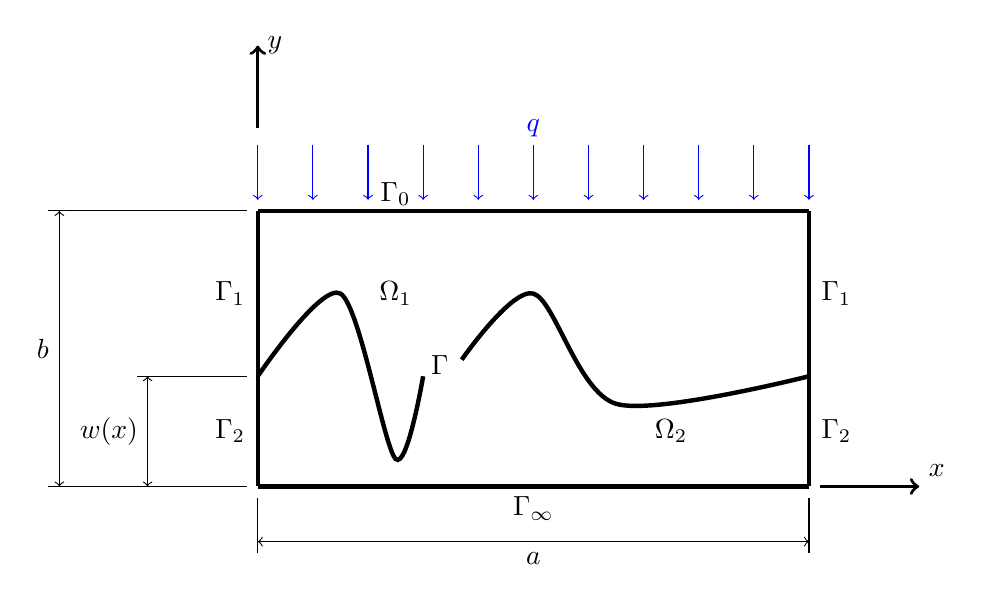
\begin{tikzpicture}[scale=0.7]

	\draw [ultra thick] (0, 0) -- (10, 0);
	%\draw [ultra thick] (0, 2) -- (7, 2);
	%\draw [ultra thick] (8, 2) -- (10, 2);
	\draw [ultra thick] plot [smooth] coordinates {(0, 2) (1.5, 3.5) (2.5, 0.5) (3, 2)};
	\draw [ultra thick] plot [smooth] coordinates {(3.7, 2.3) (5, 3.5) (6.5, 1.5) (10, 2)};
	\draw [ultra thick] (0, 5) -- (10, 5);
	\draw [ultra thick] (0, 0) -- (0, 5);
	\draw [ultra thick] (10, 0) -- (10, 5);
	
	\draw (2.5, 3.5) node {$\Omega_1$};
	\draw (7.5, 1) node {$\Omega_2$};	
	\draw (3.3, 2.2) node {$\Gamma$};
	\draw (-0.5, 3.5) node {$\Gamma_1$};
	\draw (-0.5, 1) node {$\Gamma_2$};
	\draw (10.5, 3.5) node {$\Gamma_1$};
	\draw (10.5, 1) node {$\Gamma_2$};
	\draw (5, -0.4) node {$\Gamma_\infty$};
	\draw (2.5, 5.3) node {$\Gamma_0$};
	\draw [blue](5, 6.5) node {$q$};
	\draw (5, -1.3) node {$a$};
	\draw (-3.9, 2.5) node {$b$};
	\draw (-2.7, 1) node {$w(x)$};
	
	\node [above right] at (12, 0) {$x$};
	\node [right] at (0, 8) {$y$};
	
	\draw [->, blue] (0, 6.2) -- (0, 5.2);
	\draw [->, blue] (1, 6.2) -- (1, 5.2);
	\draw [->, blue] (2, 6.2) -- (2, 5.2);
	\draw [->, blue] (3, 6.2) -- (3, 5.2);
	\draw [->, blue] (4, 6.2) -- (4, 5.2);
	\draw [->, blue] (5, 6.2) -- (5, 5.2);
	\draw [->, blue] (6, 6.2) -- (6, 5.2);
	\draw [->, blue] (7, 6.2) -- (7, 5.2);
	\draw [->, blue] (8, 6.2) -- (8, 5.2);
	\draw [->, blue] (9, 6.2) -- (9, 5.2);
	\draw [->, blue] (10, 6.2) -- (10, 5.2);
	
	\draw [->, very thick] (10.2,0) -- (12,0);
	\draw [->, very thick] (0, 6.5) -- (0,8);
	
	\draw [-] (0, -0.2) -- (0, -1.2);
	\draw [-] (10, -0.2) -- (10, -1.2);
	\draw [<->] (0, -1) -- (10, -1);
	
	\draw [-] (-0.2, 0) -- (-3.8, 0);
	\draw [-] (-0.2, 5) -- (-3.8, 5);
	\draw [-] (-0.2, 2) -- (-2.2, 2);
	\draw [<->] (-3.6, 0) -- (-3.6, 5);
	\draw [<->] (-2.0, 0) -- (-2.0, 2);

\end{tikzpicture}
\caption{Geometria do problema físico}
\label{fig2}
\end{center}
\end{figure}

Considera-se então um corpo de prova ($\Omega$) de seção transversal retangular composto por dois materiais ou regiões isotrópicas ($\Omega_1$ e $\Omega_2$), com
condutividades térmicas correspondentes $k_1$  e $k_2$, colocados em contato,
criando uma interface $\Gamma$ na qual se assume a existência de uma CTC variável com a posição $h_\Gamma(x)$.
As superfícies laterais ($\Gamma_1$ e $\Gamma_2$) das duas camadas são mantidas isoladas termicamente;
a superfície inferior ($\Gamma_\infty$) é submetida a uma temperatura prescrita; a superfície superior ($\Gamma_0$) é submetida
a um fluxo de calor por unidade de área $q$. A interseção de qualquer plano paralelo ao plano coordenado $xy$ com a interface $\Gamma$ gera uma
curva descrita por uma equação da forma $y = w(x)$.

Resumidamente, as seguintes hipóteses simplificadores foram adotadas:
\begin{itemize}
  \item O problema de condução de calor sobre o corpo de prova é em regime estacionário: $\displaystyle\frac{\partial T}{\partial t} = 0$;
  \item As condutividades térmicas $k_1$ e $k_2$ dos materiais são constantes;
  \item A variação espacial da CTC é unidimensional: $h_c \equiv h_c(x)$;
  \item O fluxo de calor $q$ sobre a superfície superior $\Gamma_0$ é constante e uniformemente distribuído;
  \item Não há dependência dos campos de temperatura com a componente $z$, ou seja, $T \equiv T(x, y)$; e
  \item Condição de contorno de terceiro tipo, ou de Robin, na interface $\Gamma$:
  		\begin{equation*}
  			-k_1\frac{\partial T_1}{\partial \mathbf{n}_1} = h_c(T_1 - T_2),
  		\end{equation*}   
\end{itemize} 
onde
$\mathbf{n}_1$ é o vetor normal à superfície $\Gamma$ e apontando para fora da região $\Omega_1$, e $T_1$ e $T_2$ são as temperaturas
correspondentes respectivamente às camadas $\Omega_1$ e $\Omega_2$, verificadas na interface $\Gamma$.

\subsection{Formulação matemática do problema direto}\label{sec_formulacao_direta}
Com base nas observações anteriores, podemos formular o problema direto de condução de calor em regime permanente através do corpo de prova $\Omega$ como segue: 

\begin{subequations}
\begin{alignat}{2}
	& \nabla^2 T_1 = 0 \quad\quad\quad\quad\quad && \text{ em } \Omega_1 \label{harm_T1} \\ \nonumber \\
	& -k_1 \frac{\partial T_1}{\partial\mathbf{n}_1} = q && \text{ em } \Gamma_0  \label{cc_T1_2} \\ \nonumber \\
	& \frac{\partial T_1}{\partial \mathbf{n}_1} = 0 && \text{ em }  \Gamma_1 \label{cc_T1_1} \\ \nonumber \\
	& -k_1 \frac{\partial T_1}{\partial\mathbf{n}_1} = h_c(T_1-T_2) \quad\quad\quad\quad\quad\quad\quad\quad && \text{ em }  \Gamma \label{cc_grad_T1} \\ \nonumber \\
	& \nabla^2 T_2 = 0 && \text{ em }  \Omega_2 \label{harm_T2} \\ \nonumber \\
	& \frac{\partial T_2}{\partial \mathbf{n}_2} = 0 && \text{ em }  \Gamma_2 \label{cc_T1_3} \\ \nonumber \\
	& T_2 = 0 && \text{ em }  \Gamma_\infty \label{cc_T1_4} \\ \nonumber \\
	& k_2\frac{\partial T_2}{\partial\mathbf{n}_2} = - k_1\frac{\partial T_1}{\partial\mathbf{n}_1} && \text{ em }  \Gamma \label{cc_T1_5}
\end{alignat}
\end{subequations}

A atribuição do valor zero à temperatura na superfície inferior $\Gamma_\infty$ do corpo $\Omega_2$, ao invés do valor prescrito, é uma simplificação
que permite a homogeinização da condição de contorno \eqref{cc_T1_4}. De fato, representando o valor da temperatura prescrita nessa superfície como $T^\star$,
o campo de temperaturas na região $\Omega_2$ seria dado por
\begin{equation}
	T_2^\star = T_2 + T^\star
\end{equation}
